
\section{Electroencephalography}
    \subsection{Brain electrical signal}
    Brain is an extremely important organ that exists in all vertebrates and most invertebrates that living on planet Earth. Enveloping the brain is a complex layer of cranium and the mandible as known as the skull located in the cranial cavity, usually near the other sensory organs, such as visual, auditory, gustatory, olfaction and equilibrioception. Brain is an extremely complex organ, the human brain has over 86 billion neurons, and each connects to thousands of others to create a network. This extraordinary network expresses that it is a very effective system. In order to transmit the signal between neurons over synapses at a very high speed to make its efficiency and fast connection, the signal that neural generates for contacting each other is basically nothing else but electrical signal.
    
        \begin{figure}[h]
        \centering
        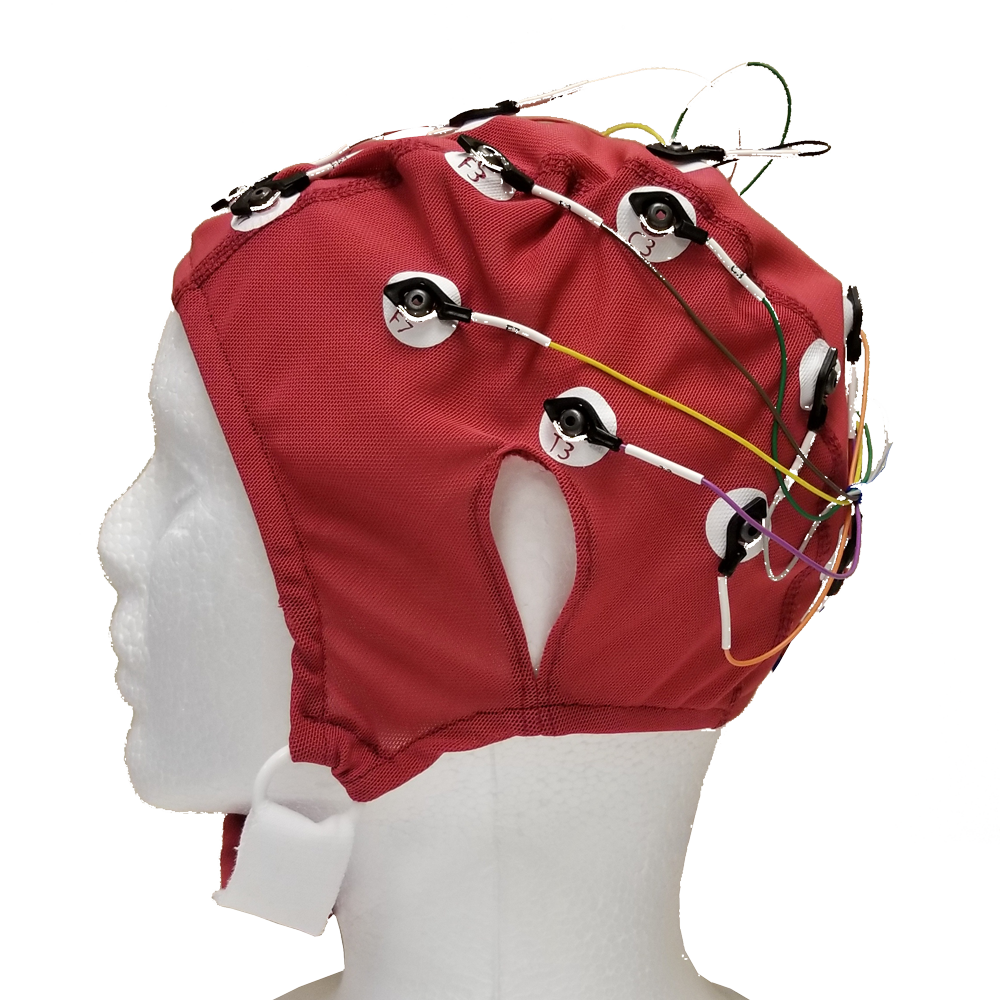
\includegraphics[width=0.3\textwidth]{images/19E.png}
        \caption{An example of tool to record the brain electrical signal}
    \end{figure} 
    
    \subsection{Electroencephalography}
    
     EEG is an method to record the neural oscillations of the brain and illustrate the operation of the body of human by that electrical signals. A different region of the brain and a different of body's activity produce a different type of EEG signal. Thus, in almost any scenario of recording EEG, one recorder cannot illustrate the whole status of the brain, but we have to create a matrix of multiple electrodes to record multiple zone in the brain. Each place in the head will generate a different signal and to be more specific, the electrode map has been normalized and use seamlessly all around the world. Furthermore, each recorder has it's own name in order to specify the region that it records. 
    
   
    
    The human brain divide into 5 main sections, and each has a specific roll to control the body both physical and mental:
    
    \begin{itemize}
        \item Frontal lobe (F) (Red)
        \item Cerebellum (C) (Cyan)
        \item Parietal lobe (P) (Yellow)
        \item Occipital lobe (O) (Emerald)
        \item Temporal lobe (T) (Green)
    \end{itemize}
    
    \begin{figure}[h]
        \centering
        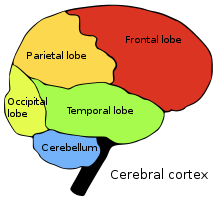
\includegraphics[width = 0.3\textwidth]{images/Brain.png}  
        \caption{Region of the brain}
        \label{fig:region_of_the_brain}
    \end{figure}
    
    Each of these regions produce different signal and if there is any skew on the place to set the electrode, it will have the wrong result. The figure below show the name and the places to put electrode on the skull. As you can see, figure 2.3 illustrates the full scale of electrode map. However, to simplify this case, The number of electrodes that we use can also can be reduced to 19 electrodes map as the figure 2.4.

    \begin{figure}
    \centering
    \begin{minipage}{.5\textwidth}
      \centering
      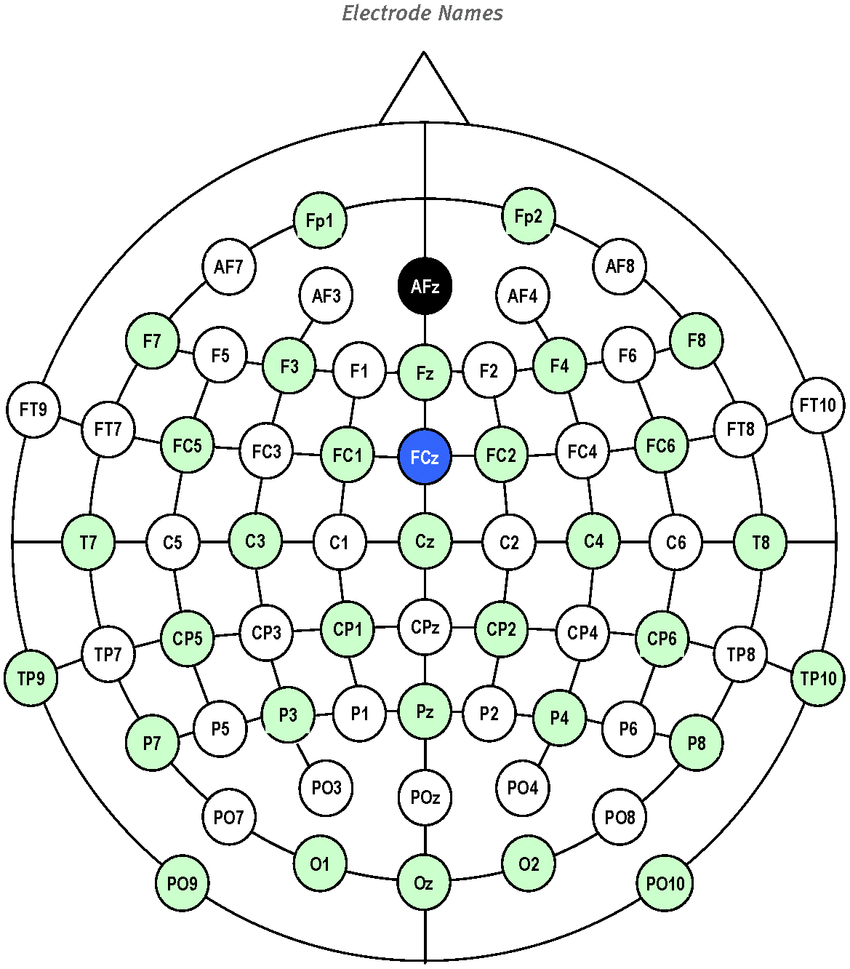
\includegraphics[width=.6\linewidth]{images/EEG_electrodes_map_full.png}
      \captionof{figure}{Full electrode map}
      \label{fig:fulle}
    \end{minipage}%
    \begin{minipage}{.5\textwidth}
      \centering
      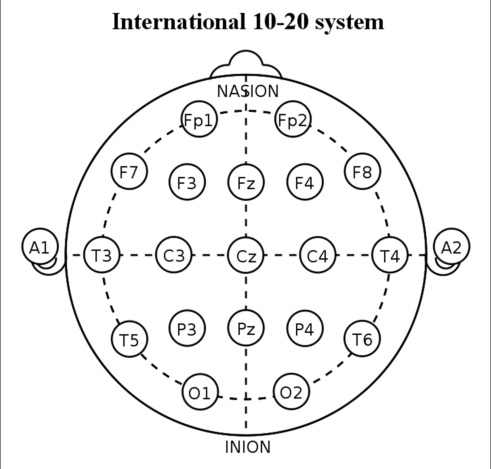
\includegraphics[width=.7\linewidth]{images/EEG_electrodes_map_19.png}
      \captionof{figure}{19 electrodes map}
      \label{fig:19e}
    \end{minipage}
    \end{figure}

    Electrode when recording the EEG signal it is contained not just only the signal, but also the noise from an extremely noisy environment. Only very tiny electric field or other electronic devices can affect how the recording process of electrode. Beside the noise come from the recording equipment itself and equipment from the surrounding area, Inside human body, some of the organ also generate electrical signal and it affects the final result. The most significant example of the organs that also create electric is our heart and our eyes. Heart beats and blinking also affect the EEG signal. Electrocardiography( heart signal) and electrooculography ( eyes signal) is the name of these two.

    The figure below demonstrates a typical 19-electrode system. As you can see, in each point of the electrode, the signal tends to be oscillate over an average line. But with the noise include, there is places that peak and not arrange in the average line and we need to get rid of them. We need a good filter to remove the noise otherwise it will make a bad approach to final data before apply machine learning technique in the signal.

    \begin{figure}[h]
        \centering
        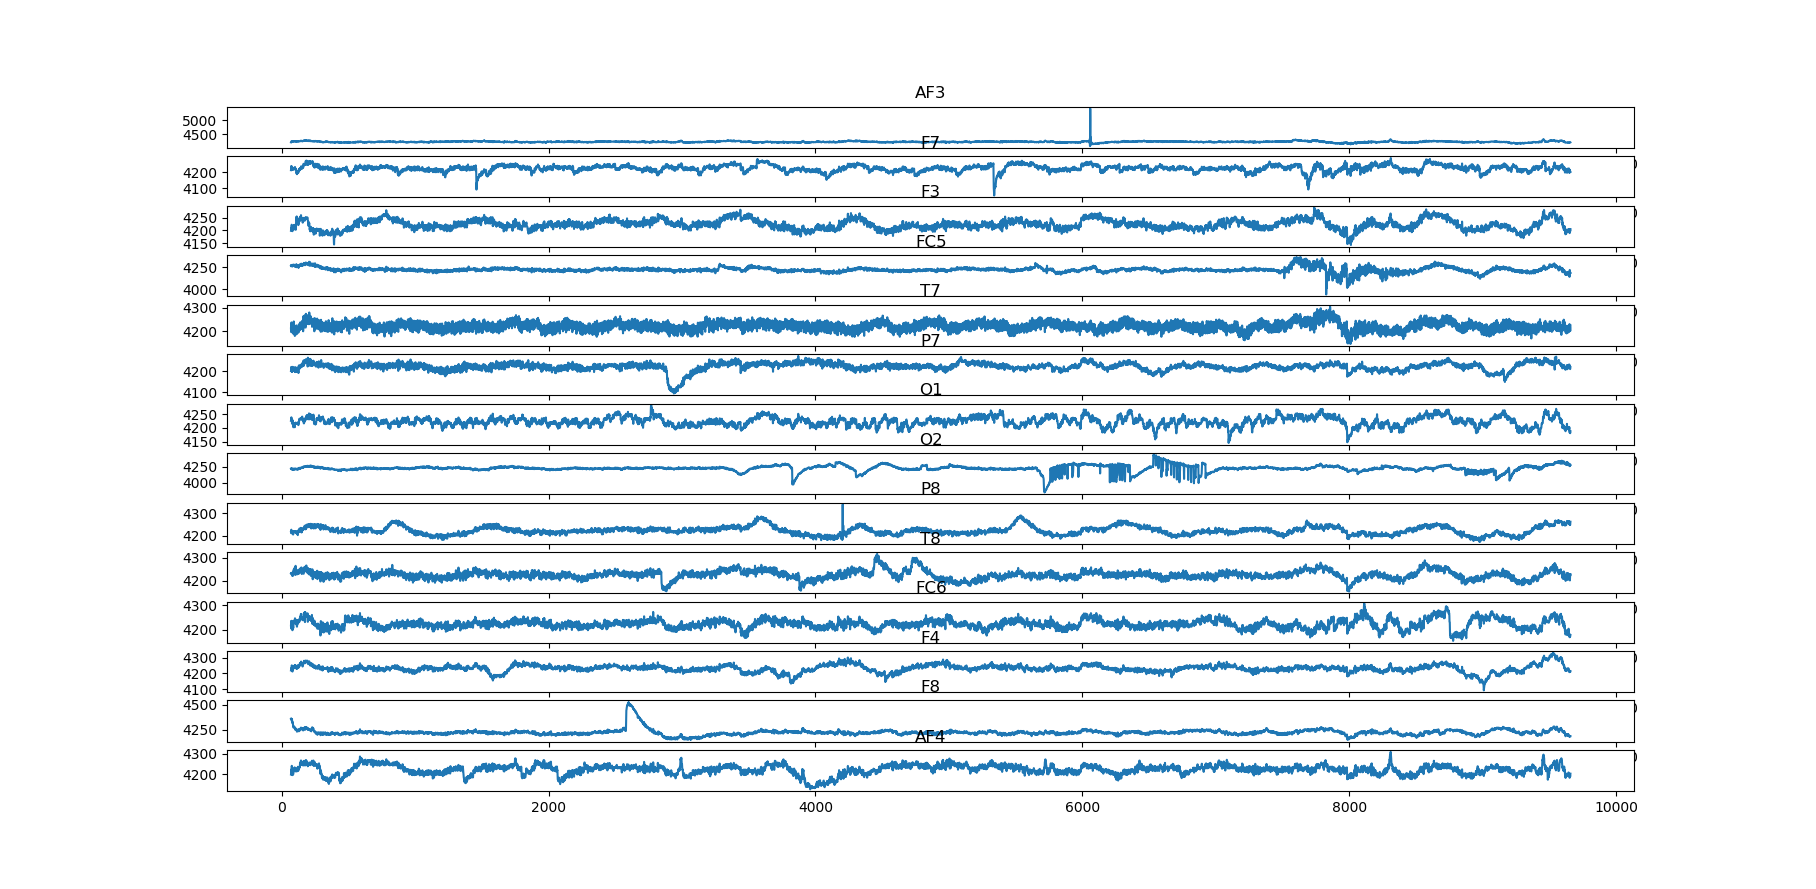
\includegraphics[width=1\textwidth]{images/EEGExample.png}
        \caption{Example of a typical EEG signals}
    \end{figure} 
    
\section{Apply machine learning in EEG signal}
    There are several types of machine learning to process the signal after all the noise be cleaned. For example, people can use neural network, Bayesian classifier, clustering and more. Even before applying machine learning method in the data we have, to be more accurate, It is also can use some technique to reduce the nodes by using nature-inspired algorithms like Genetic Algorithms (GA) and Simulating Annealing (SA)~\cite{EEG}. However, in this article, I will focus on using neural network to map the region of the brain we have with specific brain signal.
    
    It is important to know that the signal we have belong to the what part of the brain. So in this thesis I will focus using neural network to classify the 4 main region as I have cite in the subsection 1.1.2. Region P and O are very close so I will make it 1 class.
    
    \begin{itemize}
        \item Class 1: Frontal lobe (F)
        \item Class 2: Cerebellum (C)
        \item Class 3: Temporal lobe (T)
        \item Class 4: Parietal lobe (P) and Occipital lobe (O)
    \end{itemize}    
    
    \begin{figure}[h]
        \centering
        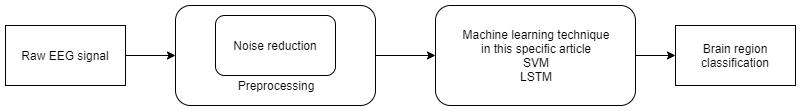
\includegraphics[width=1\textwidth]{images/GeneralDiagram.png}
        \caption{General diagram of a signal based region classification system.}
    \end{figure}
    
    The figure above illustrates the process that we will use to make the Raw EEG signal to the output is the classes mapping with the brain regions that we listed before.